\subsection{DRL-enhanced Behaviour-based Method}

In \cite{johns2018intelligent}, R. Johns proposed a method to enhance behaviour-based formationc control with deep reinforcement learning.
In this work, the bahaviour-based method proposed by Balch and Arkin \cite{balch1998behavior} is used as a comparison baseline and also the base from which the reinforment learning algorithms started their training. 

\subsubsection{Framework}

In this method, the reinforment learning network starts with the behaviours of the traditional formation control algorithm, output a action vector $F_{i,rl}$, which is represented as a vector of forces applied to agent $i$ to move.
Then the final control vector $F_{i,control}$ is caculated as a combinition of the behaviour-based control algorithm's force $F_{i,bb}$ and $F_{i,rl}$. 
A single DRL model is used by all agents, as described in the section Parameter Sharing in \cite{johns2018intelligent}, and displayed in Figure \ref{fig:drlbbmparamsharing}.

\begin{figure}
	\centering
	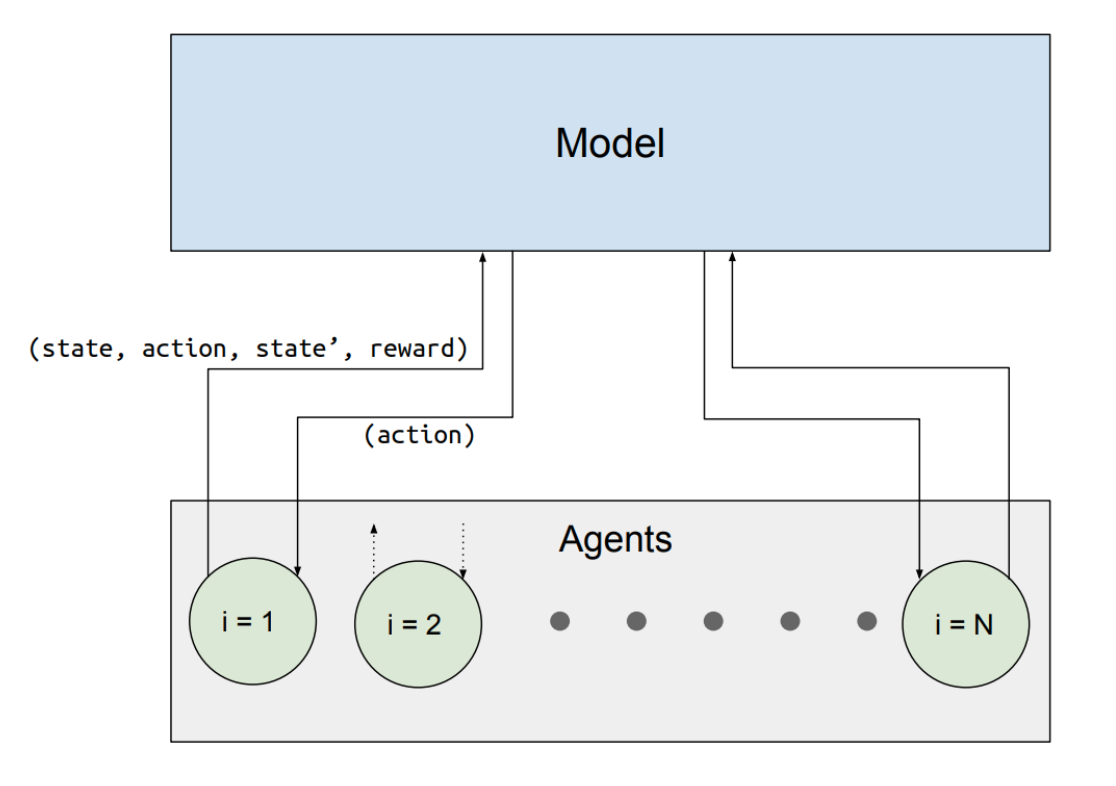
\includegraphics[width=5in]{drlbbmparamsharing.png}
	\caption{The parameter shared DRL model used by all agents.}
	\label{fig:drlbbmparamsharing} 
\end{figure}

The algorithm is implemented using OpenAI's Baselines package \cite{dhariwal2017openai}, which is a set of state-of-the-art Python implementations of reinforcement learning algorithms running on top of Tensorflow.

\subsubsection{State Representation}

In the experiment of this method, each agent is equipped with 8 range sensors, and each lidar sensor is able to recognise if an obstacle or a neighbor agent is being observed. 
And the distance data is converted to sensor power based on a value mapping function as shown in Figure \ref{fig:sensorpower}.

\begin{figure}
	\centering
	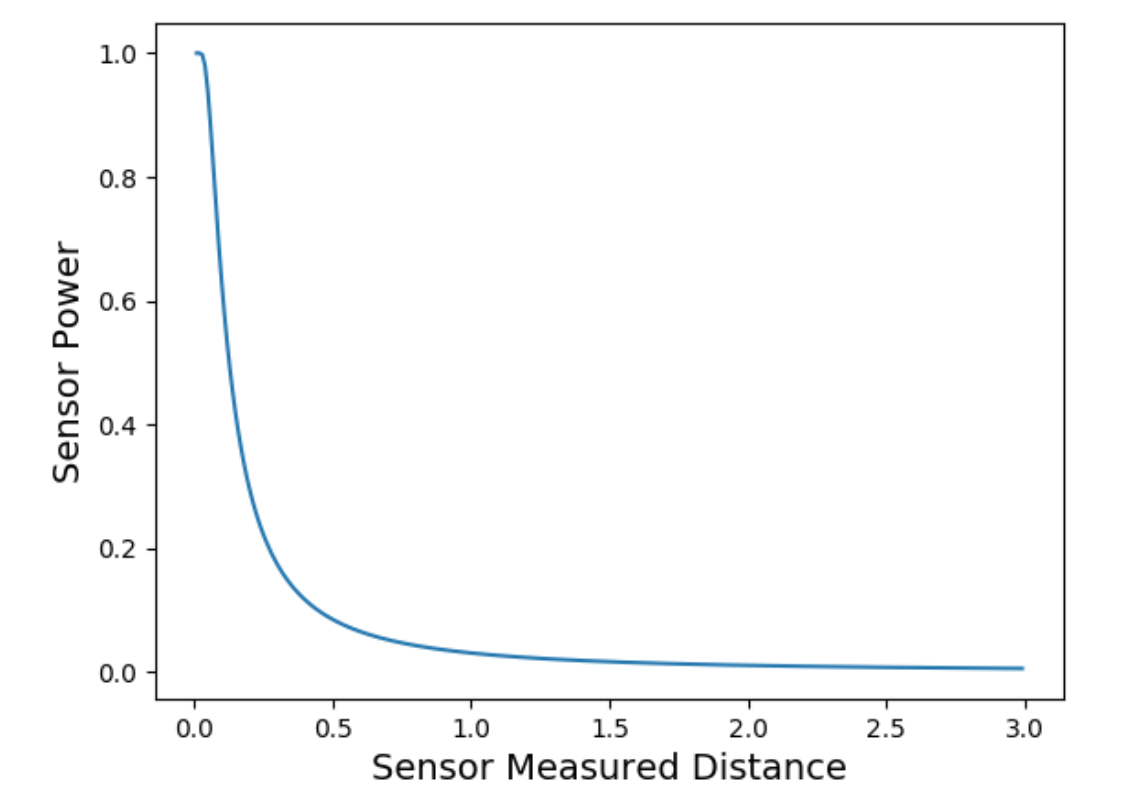
\includegraphics[width=5in]{sensorpower.png}
	\caption{The relationship between the distance measured by a sensor and the sensor’s power in an agents state space.}
	\label{fig:sensorpower} 
\end{figure}

\subsubsection{Reinforcements}

The reward function is composed by four reward parts according to Equation \ref{eq:drlbbreward}.

\begin{equation}
R=R_{ARG}+R_{GRG}+R_{OC}+R_{FD}
\label{eq:drlbbreward}
\end{equation}

\begin{compactenum}
	\item $R_{ARG}$, i.e. Agent Reached Goal, is given to an agent reaching the goal.
	\item $R_{GRG}$, i.e. Group Reached Goal, is awarded to the entire group if one group member reaches the goal.
	\item $R_{OC}$, i.e. Obstacle Collision, added to teach agents to avoid obstacles.
	\item $R_{FD}$, i.e. Formation Displacement, defined as the negative average sum of all agents' formation displacement.
\end{compactenum}

\subsubsection{Experiment}

Expriment is carried on in a 2D simulation map, which is built with the help of OpenAI gym \cite{brockman2016openai}, and obstacles are represented black circles, and agents blue, shown in Figure \ref{fig:drlbbexperiment}.

\begin{figure}
	\centering
	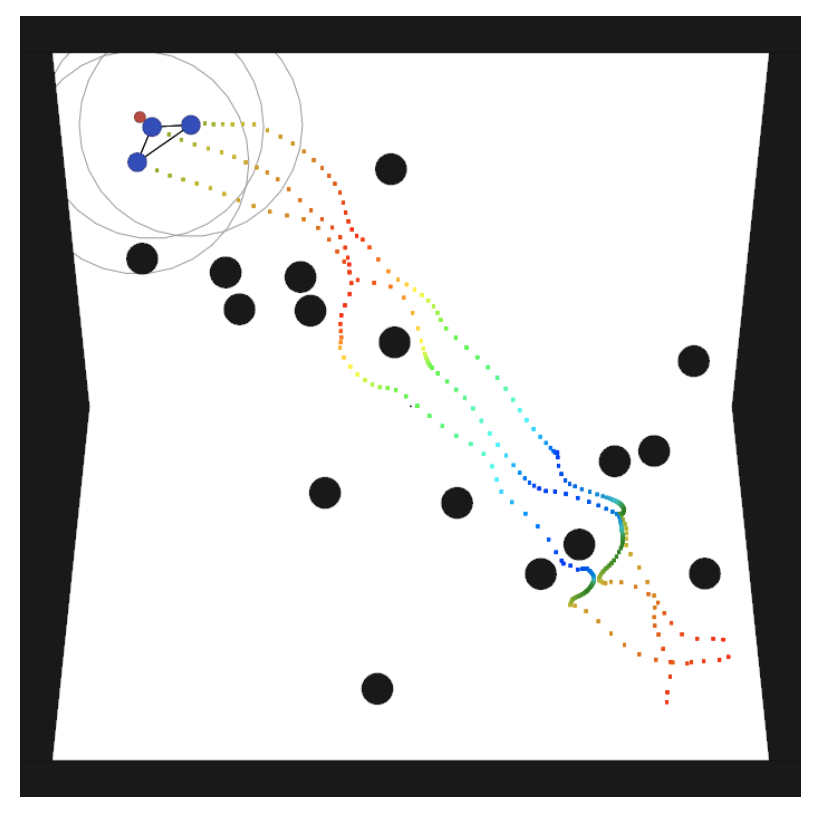
\includegraphics[width=5in]{drlbbexperiment.png}
	\caption{The experiment simulation environment of DRL-enhanced bahaviour-based method.}
	\label{fig:drlbbexperiment} 
\end{figure}

This work also establishes five evaluation metrics:

\begin{compactenum}
	\item Path Ratio. 
	The ratio of the average distance traveled by the agents divided by the Euclidean distance between the start and end point.
	\item Obstacle Collision Frequency. 
	Proportion of time the agents were in contact with an obstacle. 
	A value of zero would imply no agent ever touched an obstacle during the episode, whereas a value of one would indicate that every agent was constantly touching an obstacle during the episode.
	\item Average Formation displacement. 
	A sense of how well the algorithm were at keeping the formation could be established, which is calculated as:
	
	\begin{equation}
		E_{FD}=\frac{1}{TN}\sum_{t=0}^{T}\sum_{n=0}^{N}|x_{n,desired}(t)-x(t)|
	\end{equation}
	
	\item Success. 
	The most important measurement was the percentage of successful attempts to reach the goal. 
	Even if the goal position was not reached in a perfect formation or in the fastest time, the fact that the goal position was reached was considered crucial.
	\item Iterations to Goal. 
	To study how well the agent made use of its ability to move fast, the number of iterations needed to successfully reach the goal was monitored.
\end{compactenum}

The method is tested in 3 experiment stages:

\begin{compactenum}
	\item Fixed Obstacle Positions and Fixed Start and End Positions,
	\item Fixed Obstacle Positions with Random Start and End Positions,
	\item Random Obstacle Positions and Random Start and End Positions.
\end{compactenum}

A sample learning curve is shown in Figure \ref{fig:drlbblearningcurve}, and a sample result table in Figure \ref{fig:drlbbexperimentresult}.

\begin{figure}
	\centering
	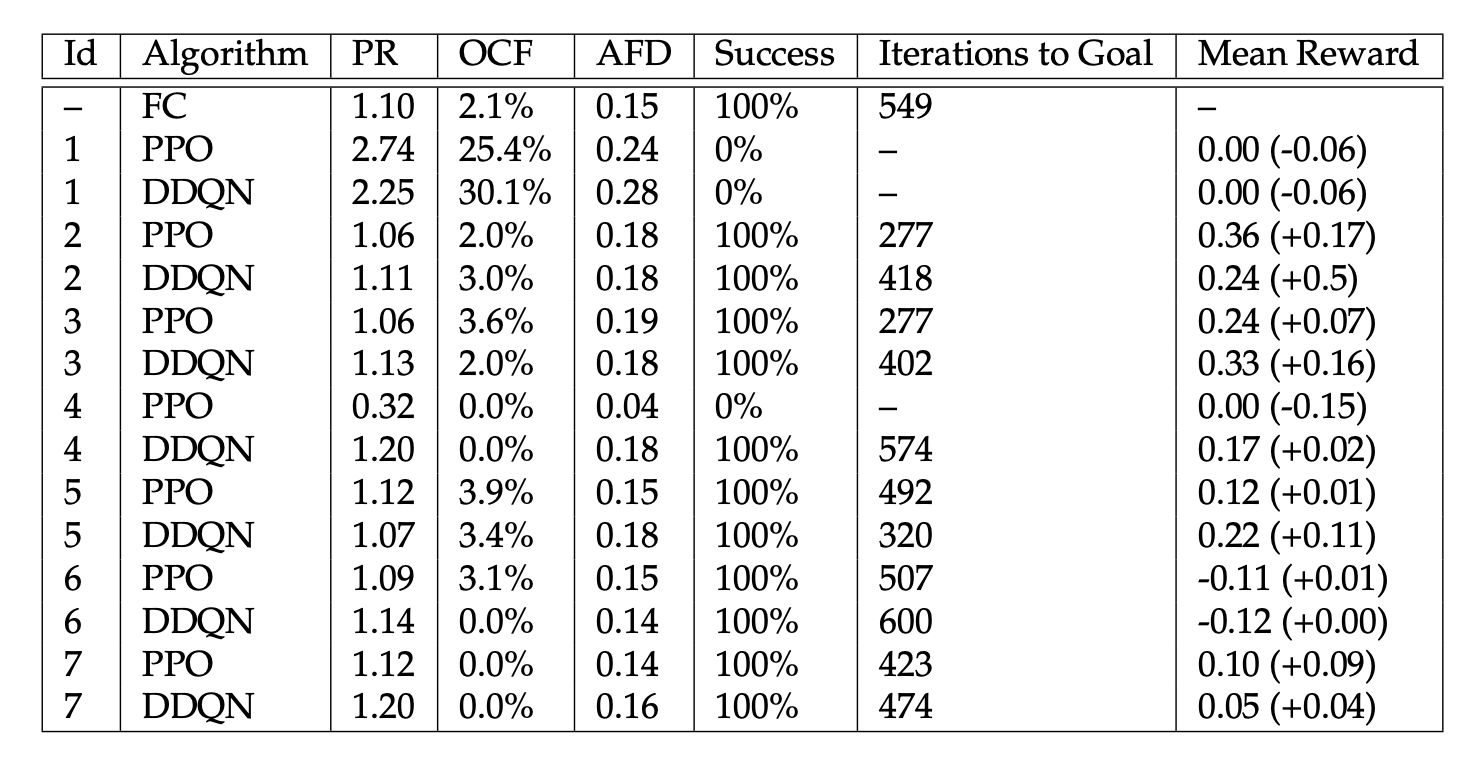
\includegraphics[width=5in]{drlbbexperimentresult.png}
	\caption{A sample result of the experiments of DRL-enhanced Behaviour-based Method.}
	\label{fig:drlbbexperimentresult} 
\end{figure}

\begin{figure}
	\centering
	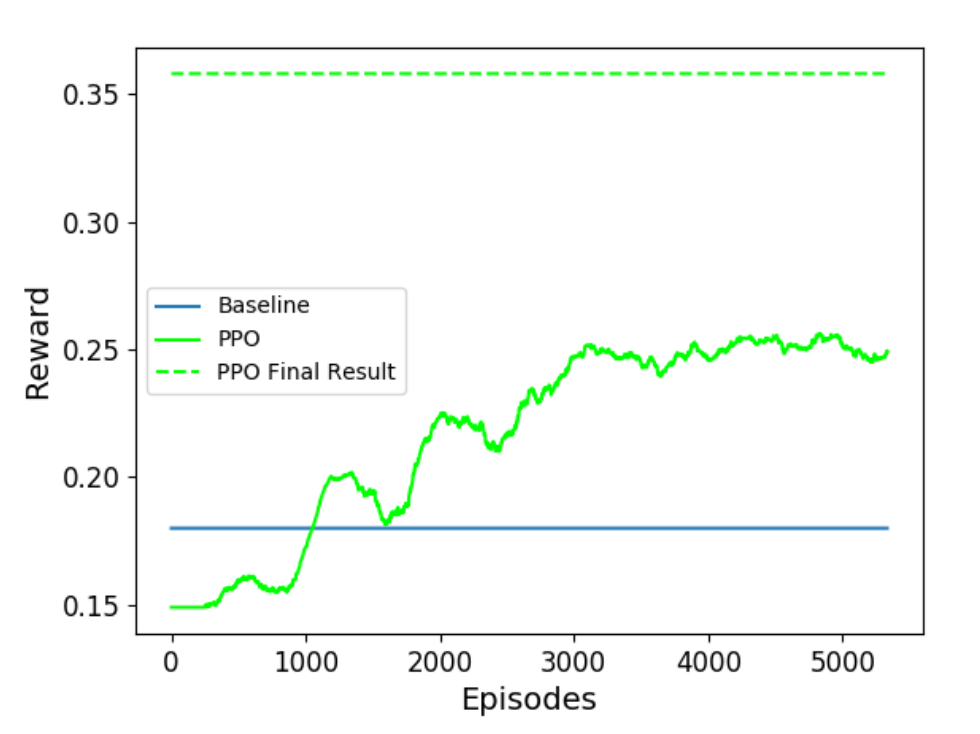
\includegraphics[width=5in]{drlbblearningcurve.png}
	\caption{A sample learning cureve of the experiments of DRL-enhanced Behaviour-based Method.}
	\label{fig:drlbblearningcurve} 
\end{figure}

\subsubsection{Discussion}

This work uses behaviour-based formation control as a base of the training of reinforcement learning network, makeing this method more stable and fast to converge.
A few shortcomings of the method can be concluded:

\begin{compactenum}
	\item The assignment problem is ignored, which means this algorithm has no capability to assign a agent to a new position in the formation during missions, and each agent can only maintain a fixed position, even swithing positions could be more efficient.
	\item The state representation, the set of 8 sensors which can recognise obstacles or neighbor agents, is a set simplified as a simulation and appears to be difficult to realise in a real-world application.
	\item This method employ deep reinforcement learning starting with behaviour-based method, makeing this method easier to train and more practical to apply, but also it introduce extra work to tune the behaviour-based method.
\end{compactenum}

